%&tex

\documentclass[14pt]{ffslides}

\ffpage{40}{1.7777}

\usepackage[english]{babel}
\usepackage[T1]{fontenc}
\usepackage{mathtools}
\usepackage{amsfonts}
\usepackage{hyperref}
\usepackage{graphicx}
\usepackage{xcolor}
\usepackage{enumitem}
\usepackage{pifont}
\usepackage{tikz}
\usepackage{tikzducks}
\usetikzlibrary{shapes,arrows,positioning,fit,circuits.logic.US}

\pagenumbering{gobble}

\newcommand{\cmark}{\ding{51}}
\newcommand{\xmark}{\ding{55}}

\geometry{
  margin=0.2cm
}

\begin{document}

\blankpage

\Huge

\ctext{0.0}{0.3}{1}{\centering\color{blue}\textbf{O Problema do Carteiro-Pato-Robô Viajante}\\
  \vskip 0.5cm
\huge MAC0318 - Introdução à Programação de Robôs Móveis}

\vskip 9cm
\begin{center}
  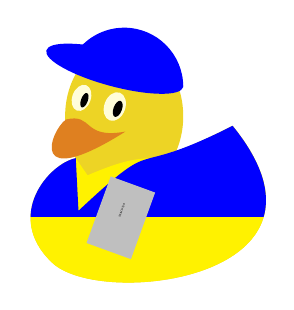
\begin{tikzpicture}[scale=1.5]
    \duck[tshirt=yellow,cap=blue,book=\scalebox{0.10}{\rotatebox{90}{\centering\color{black}\textbf{MAC0318}}},
          bookcolor=gray!50,stripes={
      \stripes[color=blue,width=1.35,distance=10,rotate=-90]
    }]
  \end{tikzpicture}
\end{center}

\newpage

\phantom{a}
\vskip 5cm
\begin{center}
  
\begin{tikzpicture}[scale=2.0]
    \duck[grumpy,xshift=-3cm,tshirt=white,jacket=black,tie=black,sunglasses=black]
    \duck[grumpy,xshift=5.25cm,tshirt=white,jacket=black,tie=black,sunglasses=black,xscale=-1]

    \duck[tshirt=white,jacket=black!95,tie=red,shorthair]
  \end{tikzpicture}
  \vskip 1cm
  \textbf{Presidente Paulo Pato}
\end{center}

\newpage

\begin{center}
  \phantom{a}
  \vskip 0.5cm
  \begin{tikzpicture}[scale=2.0]
    \duck[name=mailduck,tshirt=yellow,cap=blue,book=\scalebox{0.10}{\rotatebox{90}{\centering\color{black}\textbf{MAC0318}}},
          bookcolor=gray!50,stripes={
      \stripes[color=blue,width=1.35,distance=10,rotate=-90]
    }]
    \draw[line width=0.3cm,red] ($(mailduck-wing) + (-1,-1)$) -- ($(mailduck-wing) + (1.5,1.5)$);
    \draw[line width=0.3cm,red] ($(mailduck-wing) + (-1,1.5)$) -- ($(mailduck-wing) + (1.5,-1)$);

    \draw[line width=0.3cm] ($(mailduck-wing) + (2.5,0.5)$) -- ($(mailduck-wing) + (3.5,0.5)$);
    \draw[line width=0.3cm] ($(mailduck-wing) + (3,0)$) -- ($(mailduck-wing) + (3,1)$);

    \node at ($(mailduck-wing) + (6,0.5)$) {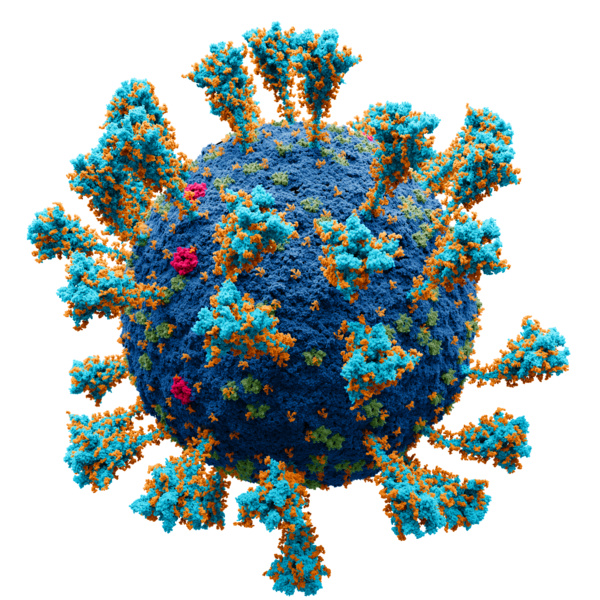
\includegraphics[width=4.5cm]{imgs/covid}};

    \duck[grumpy,yshift=-4cm,xshift=0cm,tshirt=white,jacket=black,tie=black,sunglasses=black]
    \duck[grumpy,yshift=-4cm,xshift=8.25cm,tshirt=white,jacket=black,tie=black,sunglasses=black,xscale=-1]
    \duck[laughing,yshift=-4cm,xshift=3cm,tshirt=white,jacket=black!95,tie=red,shorthair]
  \end{tikzpicture}
\end{center}

\newpage

\begin{center}
  \phantom{a}
  \vskip 0.5cm

  \begin{tikzpicture}[scale=2.0]
    \duck[name=mailduck,tshirt=yellow,cap=blue,book=\scalebox{0.10}{\rotatebox{90}{\centering\color{black}\textbf{MAC0318}}},
          bookcolor=gray!50,stripes={
      \stripes[color=blue,width=1.35,distance=10,rotate=-90]
    }]

    \draw[line width=0.3cm] ($(mailduck-wing) + (2.5,0.5)$) -- ($(mailduck-wing) + (3.5,0.5)$);
    \draw[line width=0.3cm] ($(mailduck-wing) + (3,0)$) -- ($(mailduck-wing) + (3,1)$);

    \node at ($(mailduck-wing) + (6,0.5)$) {\def\svgwidth{3cm}\input{imgs/robot.pdf_tex}};

    \duck[grumpy,yshift=-4cm,xshift=0cm,tshirt=white,jacket=black,tie=black,sunglasses=black]
    \duck[grumpy,yshift=-4cm,xshift=8.25cm,tshirt=white,jacket=black,tie=black,sunglasses=black,xscale=-1]
    \duck[laughing,yshift=-4cm,xshift=3cm,tshirt=white,jacket=black!95,tie=red,shorthair]
  \end{tikzpicture}
\end{center}

\newpage

\begin{center}
  \phantom{a}
  \vskip 0.5cm

  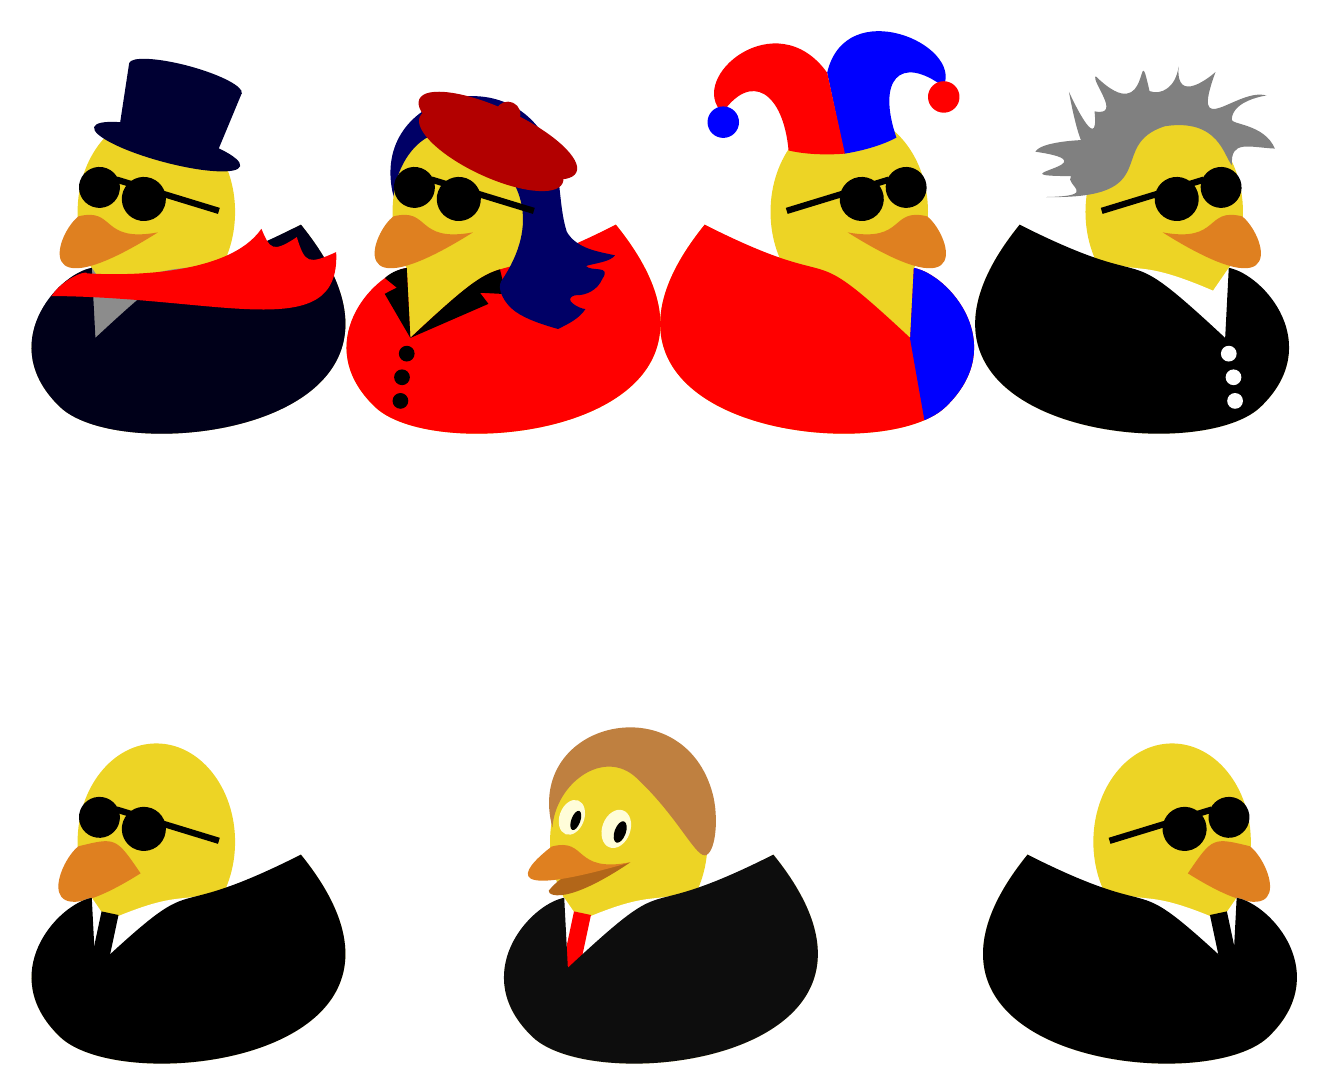
\begin{tikzpicture}[scale=2.0]
    \duck[tophat=blue!20!black,sunglasses=black,cape=red,tshirt=gray!90,jacket=blue!10!black]
    \duck[xshift=2cm,longhair=blue!40!black,sunglasses=black,beret=red!70!black,jacket=red,lapel=black,buttons]
    \duck[xscale=-1,xshift=-6.2cm,sunglasses=black,harlequin=blue,niuqelrah=red,jacket=red,stripes={\stripes[color=blue,width=0.46, distance=3]}]
    \duck[xscale=-1,xshift=-8.2cm,crazyhair=gray,jacket=black,tshirt=white,buttons=white,sunglasses=black]

    \duck[grumpy,yshift=-4cm,xshift=0cm,tshirt=white,jacket=black,tie=black,sunglasses=black]
    \duck[grumpy,yshift=-4cm,xshift=8.25cm,tshirt=white,jacket=black,tie=black,sunglasses=black,xscale=-1]
    \duck[laughing,yshift=-4cm,xshift=3cm,tshirt=white,jacket=black!95,tie=red,shorthair]
  \end{tikzpicture}
\end{center}

\newpage

\ctext{0.05}{0.05}{0.5}{\textcolor{blue}{\textbf{Informações disponíveis}}}

\begin{center}
  \phantom{a}
  \vskip 1cm
  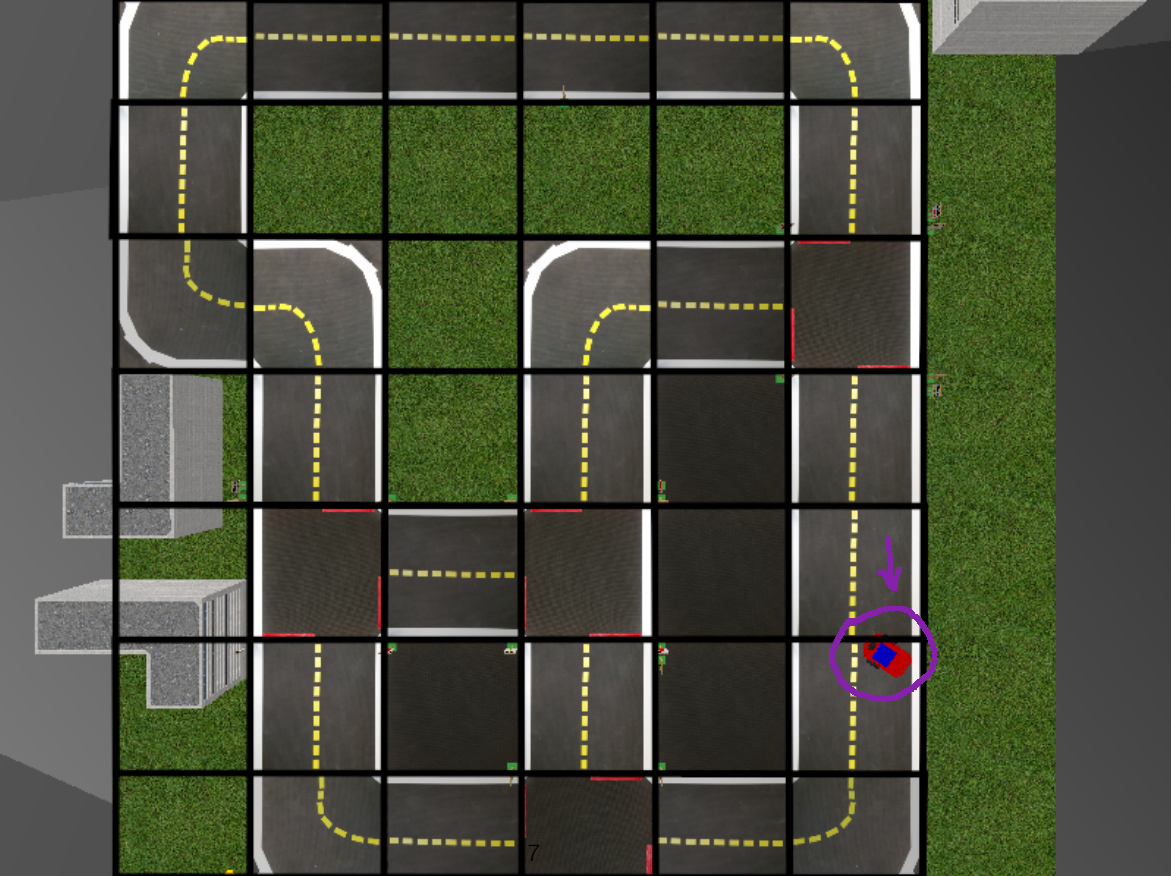
\includegraphics[height=0.8\paperheight]{imgs/init}
\end{center}

\newpage

\ctext{0.05}{0.05}{0.5}{\textcolor{blue}{\textbf{Informações disponíveis}}}

\begin{center}
  \phantom{a}
  \vskip 1cm
  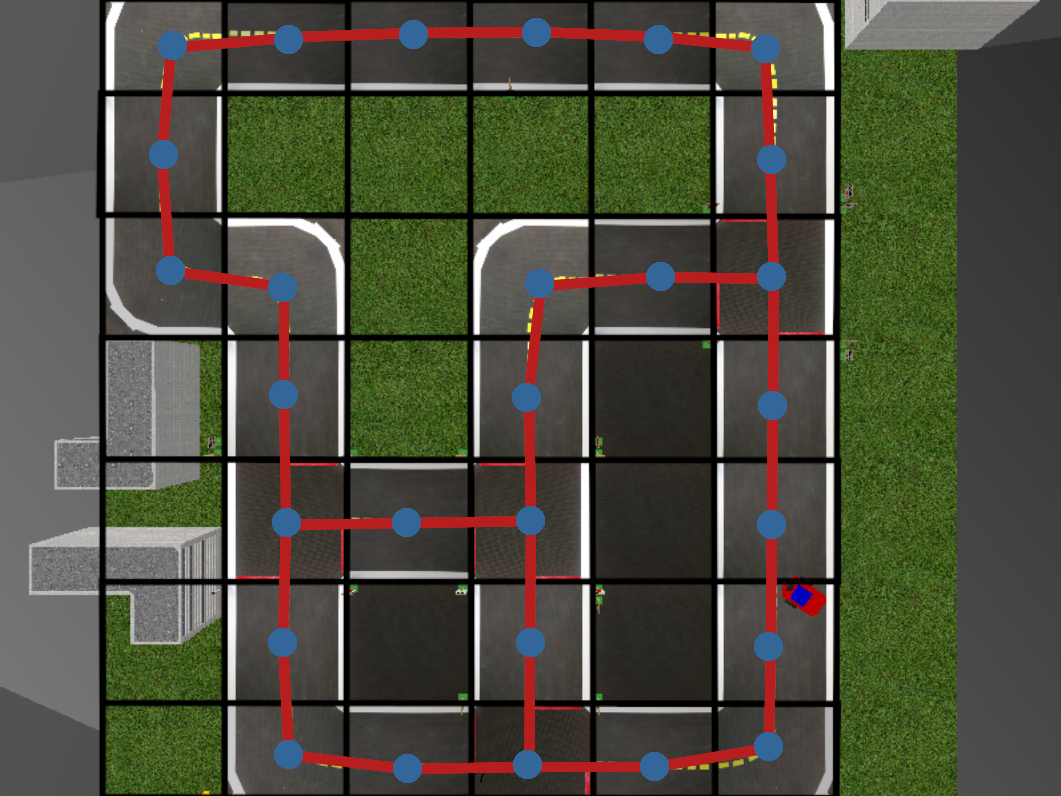
\includegraphics[height=0.8\paperheight]{imgs/graph}
\end{center}

\newpage

\ctext{0.05}{0.05}{0.5}{\textcolor{blue}{\textbf{Informações disponíveis}}}

\begin{center}
  \phantom{a}
  \vskip 1cm
  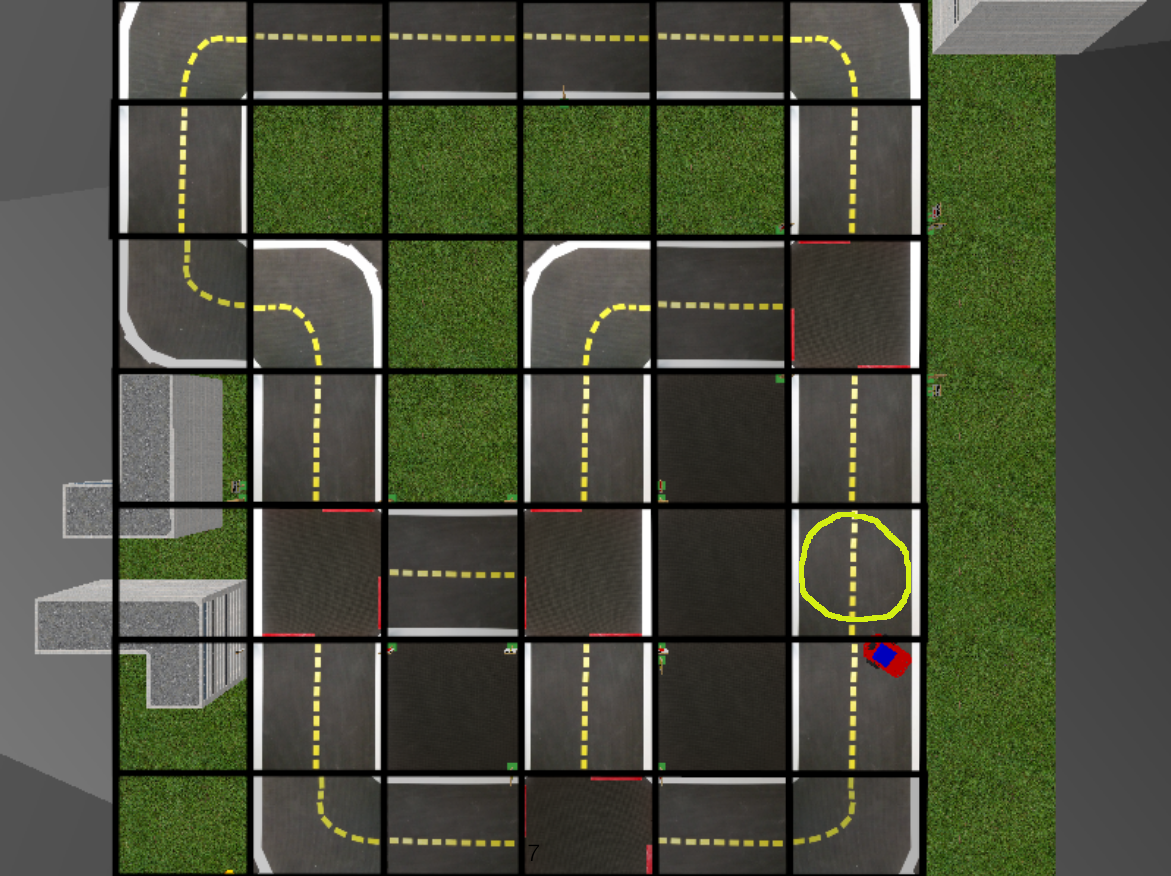
\includegraphics[height=0.8\paperheight]{imgs/delivery}
\end{center}

\newpage

\ctext{0.05}{0.05}{0.5}{\textcolor{blue}{\textbf{Leis da Pato-robótica}}}

\begin{center}
  \phantom{a}
  \vskip 1.0cm

  \begin{tikzpicture}[scale=2.0]
    \node at (1,0) {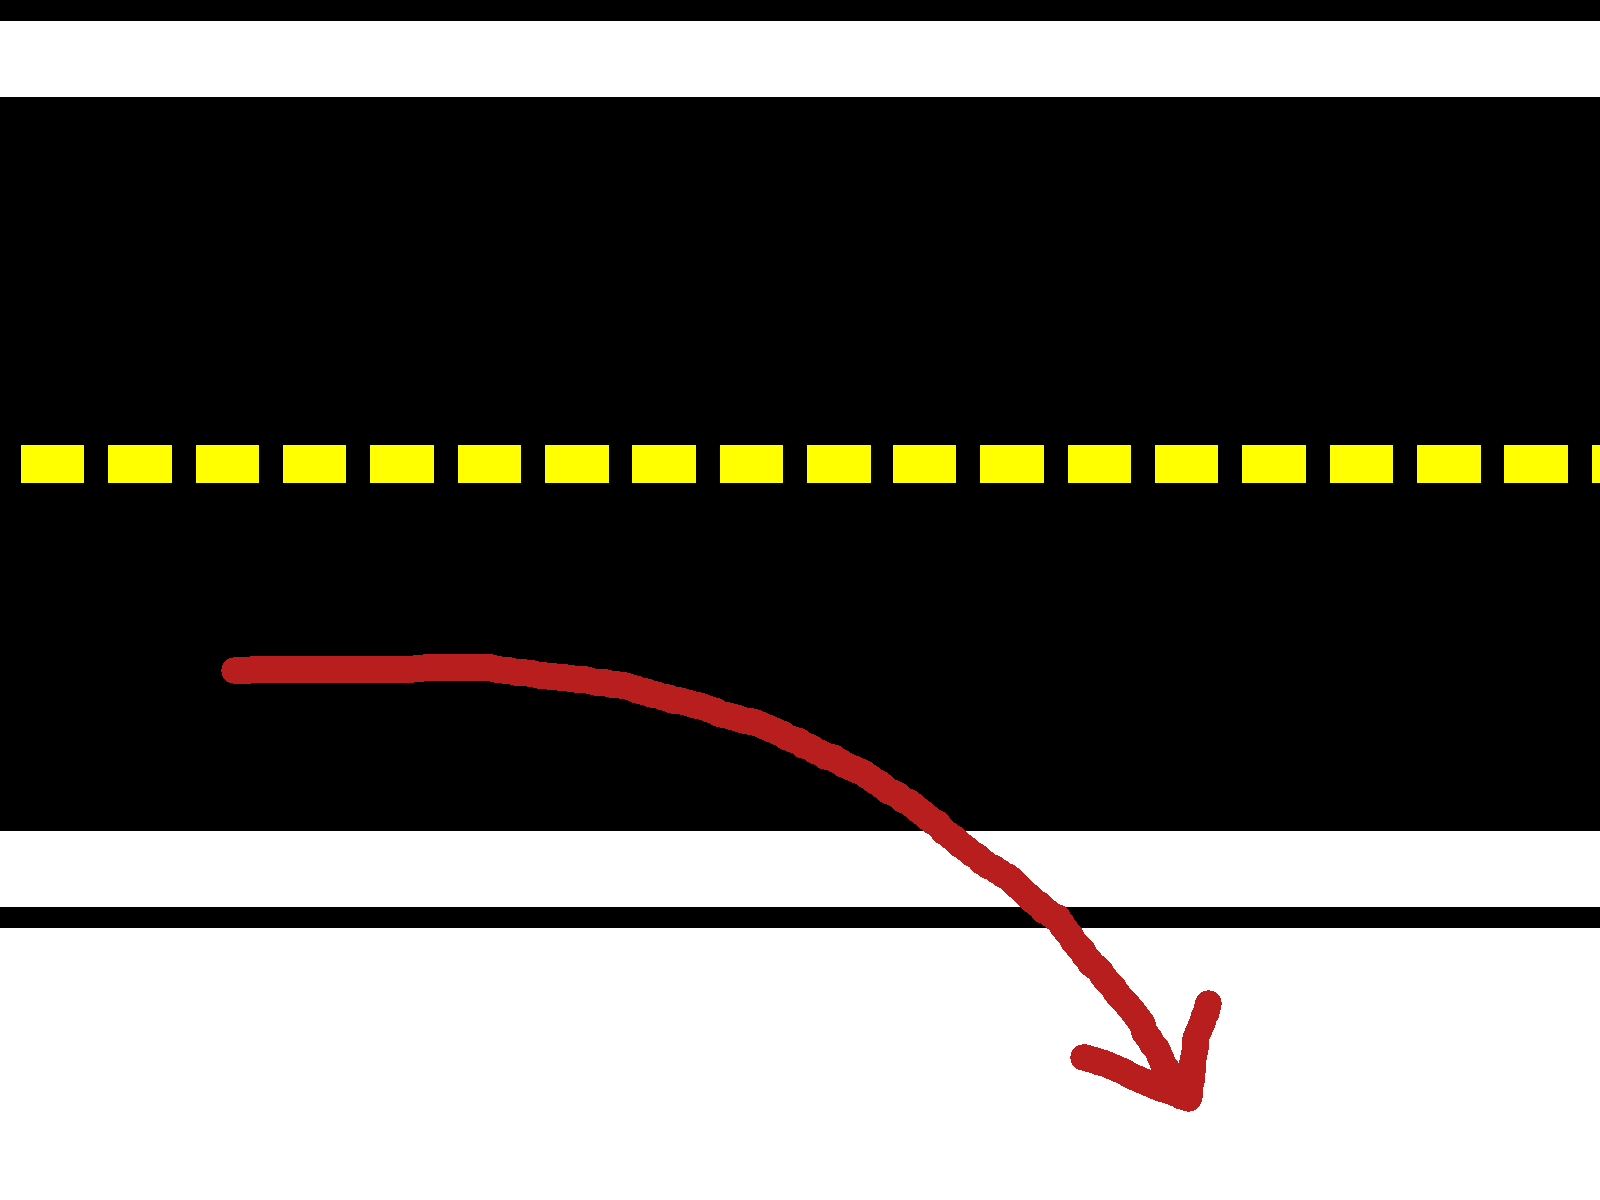
\includegraphics[height=7cm]{imgs/out}};

    \duck[grumpy,yshift=-4cm,xshift=-3cm,tshirt=white,jacket=black,tie=black,sunglasses=black]
    \duck[grumpy,yshift=-4cm,xshift=5.25cm,tshirt=white,jacket=black,tie=black,sunglasses=black,xscale=-1]
    \duck[laughing,speech={\color{red}\xmark},yshift=-4cm,tshirt=white,jacket=black!95,tie=red,shorthair]
  \end{tikzpicture}
\end{center}

\newpage

\ctext{0.05}{0.05}{0.5}{\textcolor{blue}{\textbf{Leis da Pato-robótica}}}

\begin{center}
  \phantom{a}
  \vskip 1.0cm

  \begin{tikzpicture}[scale=2.0]
    \node at (1,0) {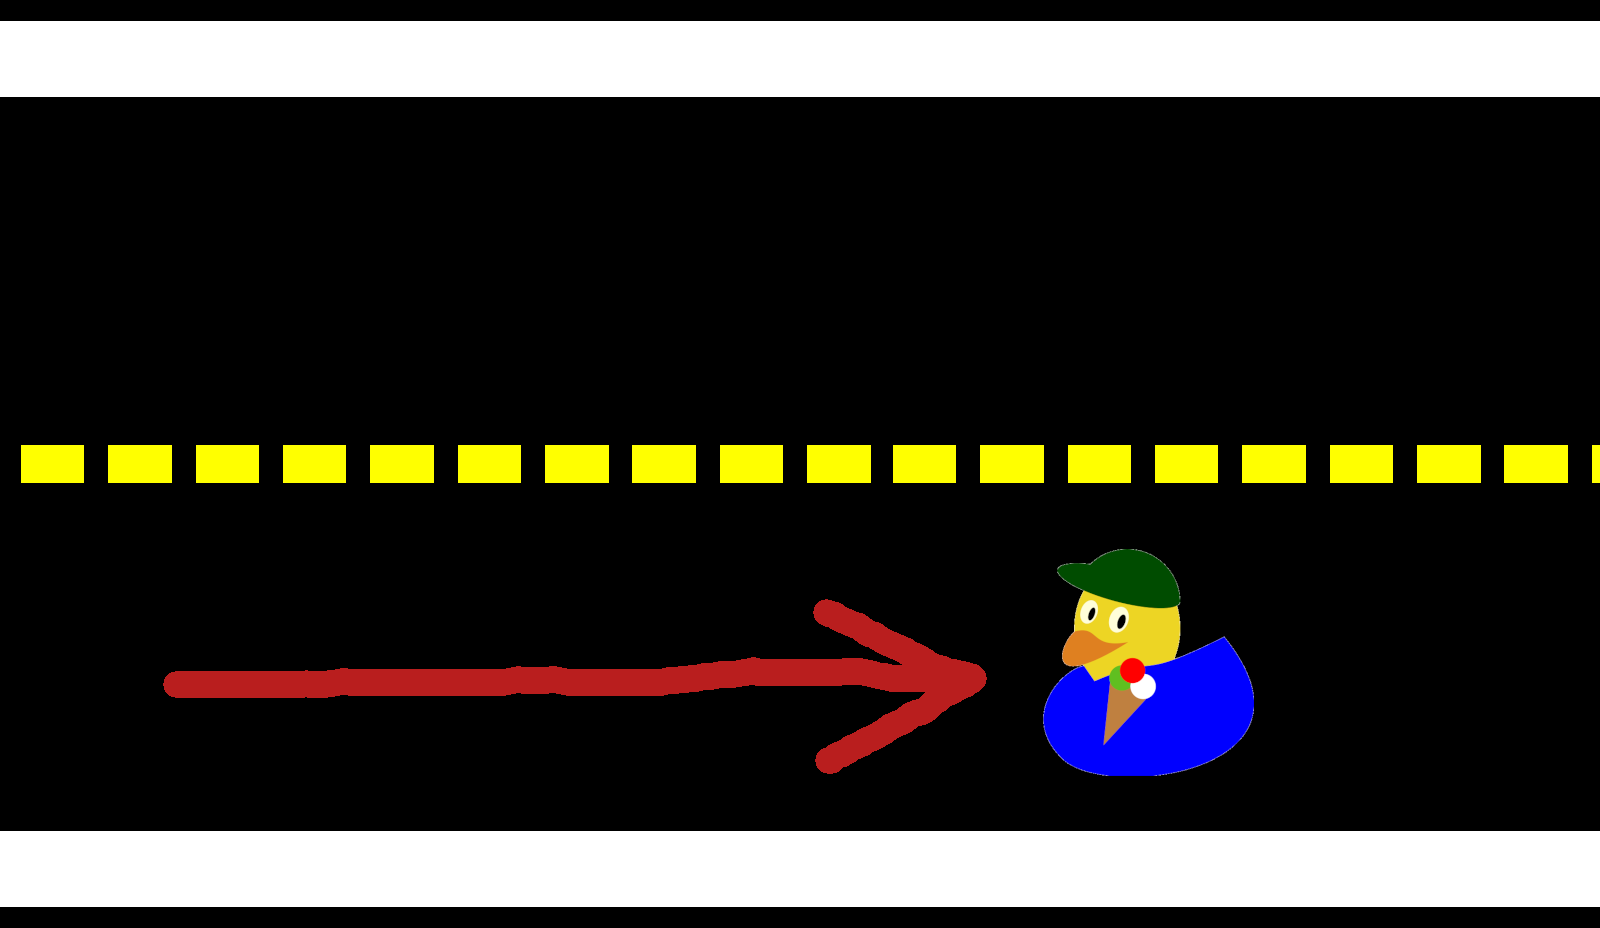
\includegraphics[height=5.5cm]{imgs/crash}};

    \duck[grumpy,yshift=-4.5cm,xshift=-3cm,tshirt=white,jacket=black,tie=black,sunglasses=black]
    \duck[grumpy,yshift=-4.5cm,xshift=5.25cm,tshirt=white,jacket=black,tie=black,sunglasses=black,xscale=-1]
    \duck[laughing,speech={\color{red}\xmark},yshift=-4.5cm,tshirt=white,jacket=black!95,tie=red,shorthair]
  \end{tikzpicture}
\end{center}

\newpage

\ctext{0.05}{0.05}{0.5}{\textcolor{blue}{\textbf{Leis da Pato-robótica}}}

\begin{center}
  \phantom{a}
  \vskip 1.0cm

  \begin{tikzpicture}[scale=2.0]
    \node at (1,0) {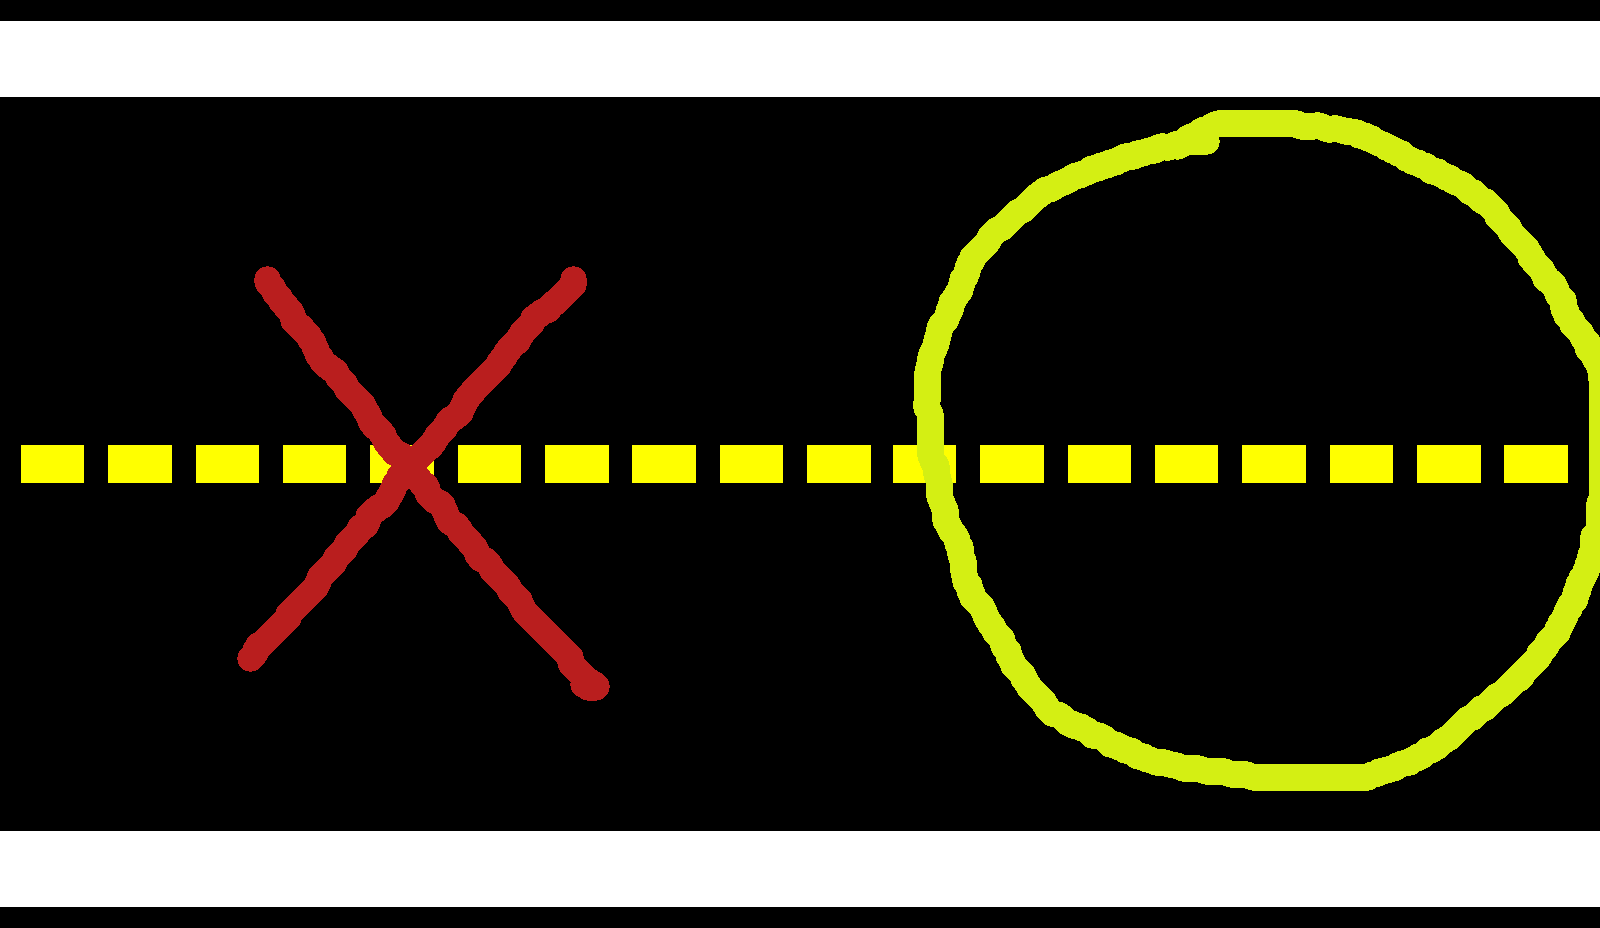
\includegraphics[height=5.5cm]{imgs/wrong}};

    \duck[grumpy,yshift=-4.5cm,xshift=-3cm,tshirt=white,jacket=black,tie=black,sunglasses=black]
    \duck[grumpy,yshift=-4.5cm,xshift=5.25cm,tshirt=white,jacket=black,tie=black,sunglasses=black,xscale=-1]
    \duck[laughing,speech={\color{red}\xmark},yshift=-4.5cm,tshirt=white,jacket=black!95,tie=red,shorthair]
  \end{tikzpicture}
\end{center}

\newpage

\ctext{0.05}{0.05}{0.5}{\textcolor{blue}{\textbf{Bônus}}}

\begin{center}
  \phantom{a}
  \vskip 1.0cm

  \begin{tikzpicture}[scale=2.0]
    \node at (1,0) {
\includegraphics[height=8.5cm]{imgs/cop26}};

    \duck[grumpy,yshift=-4cm,xshift=-3cm,tshirt=white,jacket=black,tie=black,sunglasses=black]
    \duck[grumpy,yshift=-4cm,xshift=5.25cm,tshirt=white,jacket=black,tie=black,sunglasses=black,xscale=-1]
    \duck[laughing,speech={\color{green!35!black}\cmark},yshift=-4cm,tshirt=white,jacket=black!95,tie=red,shorthair]
  \end{tikzpicture}
\end{center}

\newpage

\begin{center}
  \phantom{a}
  \vskip 5.0cm

  
\begin{tikzpicture}[scale=2.0]
    \duck[grumpy,xshift=-3cm,tshirt=white,jacket=black,tie=black,sunglasses=black]
    \duck[grumpy,xshift=5.25cm,tshirt=white,jacket=black,tie=black,sunglasses=black,xscale=-1]
    \duck[laughing,speech={\textbf{!}},tshirt=white,jacket=black!95,tie=red,shorthair]
  \end{tikzpicture}

  \vskip 1cm

  \textbf{Boa sorte e bom trabalho! Patolândia conta com vocês!}
\end{center}

\end{document}
